\documentclass[twoside]{article}

\usepackage[math]{kurier}
\usepackage[sc]{mathpazo}
\renewcommand{\sfdefault}{kurier}

\usepackage{framed} % or, "mdframed"
\usepackage[framed]{ntheorem}
\newframedtheorem{frm-def}{Definition}

\usepackage{graphicx}
\setlength{\oddsidemargin}{0.25 in}
\setlength{\evensidemargin}{-0.25 in}
\setlength{\topmargin}{-0.6 in}
\setlength{\textwidth}{6.5 in}
\setlength{\textheight}{8.5 in}
\setlength{\headsep}{0.75 in}
\setlength{\parindent}{0 in}
\setlength{\parskip}{0.1 in}


\newcounter{lecnum}
\renewcommand{\thepage}{\thelecnum-\arabic{page}}
\renewcommand{\thesection}{\thelecnum.\arabic{section}}
\renewcommand{\theequation}{\thelecnum.\arabic{equation}}
\renewcommand{\thefigure}{\thelecnum.\arabic{figure}}
\renewcommand{\thetable}{\thelecnum.\arabic{table}}


\newcommand{\lecture}[4]{
   \pagestyle{myheadings}
   \thispagestyle{plain}
   \newpage
   \setcounter{lecnum}{#1}
   \setcounter{page}{1}
   \noindent
   \begin{center}
   \framebox{
      \vbox{\vspace{2mm}
    \hbox to 6.28in { {\bf \sffamily AA 274: Introduction to Robotic Autonomy
                        \hfill Winter 2018} }
       \vspace{4mm}
       \hbox to 6.28in { {\sffamily{\Large \hfill Lecture #1 #2  \hfill}} }
       \vspace{2mm}
       %\hbox to 6.28in { {\it \hfill Scribes: #4} }
      \vspace{2mm}}
   }
   \end{center}
   \markboth{Lecture #1: #2}{Lecture #1: #2}

   \vspace*{4mm}
}



%%%%%%%%%%%%%%%%%%%%%%%%%%
%document
\begin{document}
%modify this
\lecture{2}{The Robot Operating System (ROS)}{}

\section{Introduction}

Experts in the Silicon Valley have said that we now live in a Golden Age of robotics, where high-quality hardware is both affordable and easily accessible. The developments of the past decade have enabled professionals and hobbyists alike to develop robotics from the comfort of their homes. This growth in the robotics industry is fortuitously bolstered by the existence of the Robot Operating System (ROS), a robust software introduced in this lecture.

\section{History of ROS}

The earliest versions of ROS originated with the Stanford AI Robot (STAIR) project in 2007. At this time, there existed no way for the various robotics development programs to collaborate or share work. To solve this problem, a software architect and entrepreneur named Scott Hassan attracted some of the greatest minds in robotics to create a free, open source software called the Robot Operating System. The development of ROS gained traction with the inception of Willow Garage, a software company founded by Hassan in 2006. The organization was designed to accelerate the development of non-military and open source robotics by standardizing the software frequently used in robotic tasks. Willow Garage funded ROS development until 2012, when the Open Source Robotics Foundation (OSRF) was created to support the development, distribution, and adoption of open software and hardware for use in robotics research, education, and product development. As of this day, ROS is ten years old and still maintained by the OSRF along with Gazebo, a virtual robotic simulator.

\section{What is ROS?}

Despite what its name suggests, ROS is not an operating system. The Robot Operating System can be described as a collection of tools, libraries, and conventions that aim to simplify the task of creating complex and robust robot behavior across a wide variety of platforms. At its creation, it was the combination of many existing projects such as OpenCV, Stage, Gazebo, OpenSLAM, Orocos KDL, and other ROS wrappers. Integrating ROS in one's project seldom takes more than a couple of lines of code; it can be seen simply as "gluing" components to work together. The development is mostly in a language such as Python or C++.

Although many of today's robotic platforms did not exist when Willow Garage was coming up with ROS, the developers were visionary enough to design the software to be compatible with any general robot - whether it be a flying quadcopter, a wheeled rover, or a bipedal humanoid. Early ROS developers learned that a powerful and efficient method to handle the complexity of robotic software could be accomplished using modules, as shown in Figure 2.1. This modularity takes the form of independent robotic components that perform separate functions and simplify the exchange of information. These components, called "nodes", share data with one another and act as the basic building blocks of ROS. Nodes can vary in function from sensor drivers at the low-level to even high-level tasks such as path planning with dynamic obstacle avoidance. The software design pattern used to facilitate the message exchange between nodes is known as the Publish-Subscribe (Pub/Sub) model. Within the context of this course, Pub/Sub is the communication framework that ROS relies on.

ROS is not a real-time framework; yet each of its components, ticking on the same clock, can infer the recency of a message through its time-stamp.
\begin{figure}[ht]
\centering
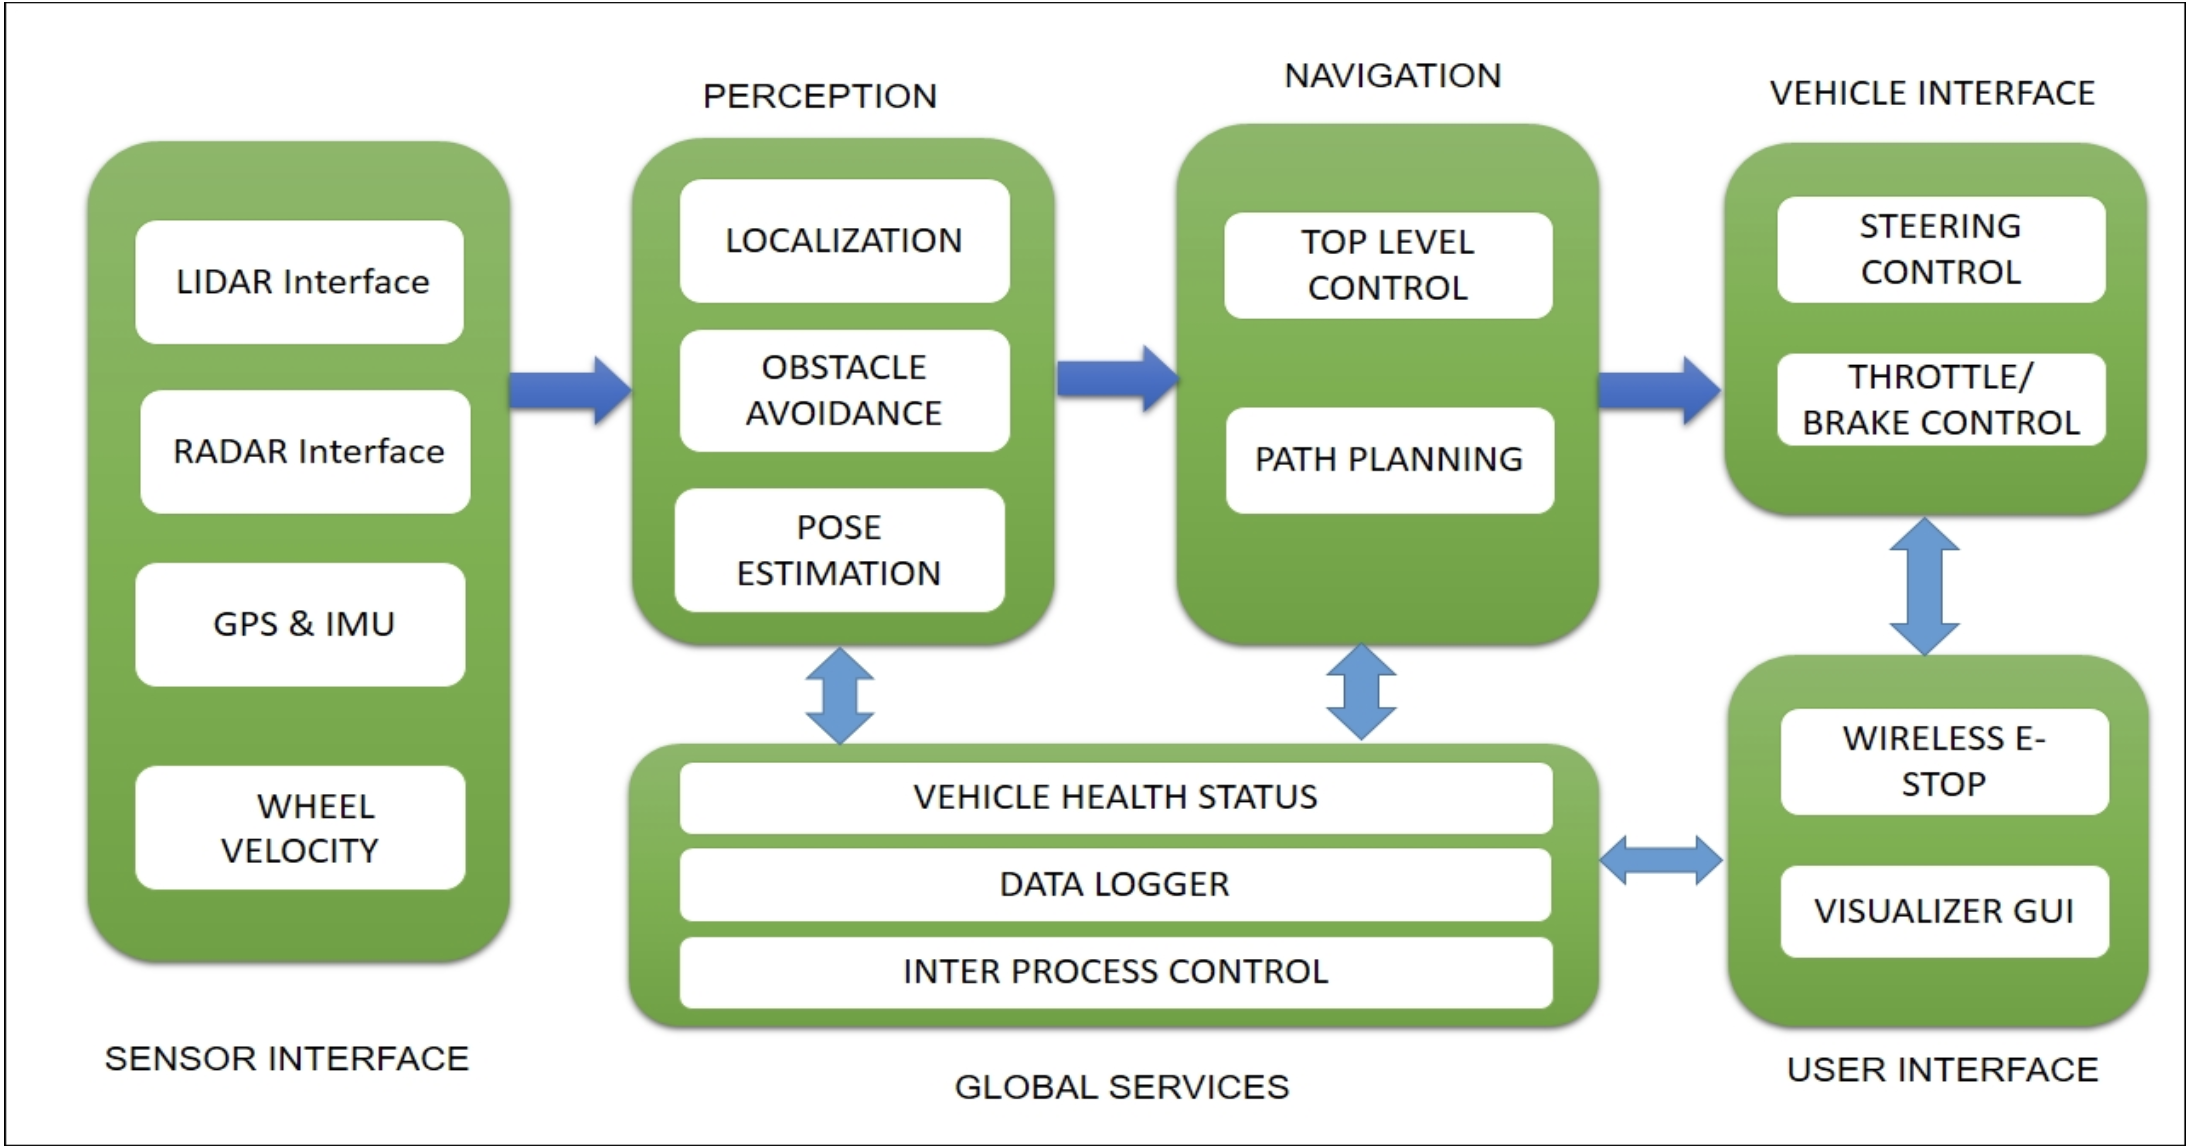
\includegraphics[width=1\textwidth]{ModularityPhoto}
\caption{Modularity designed for the complexity of robotic programming.}
\end{figure}

\section{Main Components of ROS}
The three main components of ROS with the Pub/Sub programming model are the Nodes, the Master, and the Message Types. The nodes are responsible for publishing or subscribing to certain pieces of information that are shared within a virtual "chat room" called a topic. The publisher and subscriber nodes communicate with each other via these topics to perform their functions. A separate software called the master is a process that can run on any piece of hardware to coordinate the exchange between the publishers and subscribers. It is responsible for assigning network addresses to ensure that publishers and subscribers are connected to the correct topics, even if they are running on different computers. The information is securely exchanged using message types, which serve as a powerful abstraction away from specific pieces of hardware. Using message types, nodes can read certain data types (i.e. camera image, laser scan data, motion control) in the same way regardless of hardware brand or design.

\begin{frm-def}[Master]
The master is a process that is in charge of coordinating nodes, publishers, and subscribers. There is exactly one running at any time. The master allows the nodes to find each other but is not used to send or receive messages.
\end{frm-def}

A unique feature of the master process is that is does not need to exist within the robot's hardware. The master can be facilitated remotely, on a much larger and more powerful computer and its execution is not constrained by the robotic components. Furthermore, the messages published within the topics do not go through the master; the exchange is peer-to-peer between the nodes.\\ % Add more stuff about master here.

\begin{frm-def}[Node]
A node is a process that is connected to the Pub/Sub network in ROS. Nodes communicate with each other via topics to perform tasks.
\end{frm-def}

Any system built using ROS consists of nodes, which are small parts of the larger program that work together to form a robot system. Nodes can be sensors, actuators, or simply computations that work in tandem with one another. For example, a simple system might consist of a distance sensor and a motor on a wheeled robot. If the robot wants to be some distance from a wall, the distance sensor node detects the current position and sends that information to the motor node, which acts to move the robot toward the desired position. There is no great reason that a system like that needs nodes, but suppose now the robot wants to stay centered between two walls. Adding a new sensor node for a second distance sensor is somewhat trivial. This can be further expanded to add more sensors and actuators. The node system allows the user to scale up to very complex robots by adding nodes for each additional component.\\

\begin{frm-def}[Message]
Nodes communicate with each other via peer-to-peer messages. Some common message types are camera images, laser scan data, and motion control commands.
\end{frm-def}

The peer-to-peer message system that ROS uses is illustrated in Figure 2.2. Messages contain information such as sensor data and commands. The messages (Msg) are sent over a topic. For example, sensor nodes send messages to various topics, which controller nodes access to send commands to motors and actuators to move the robot or perform some other action.\\

\begin{figure}[ht]
\centering
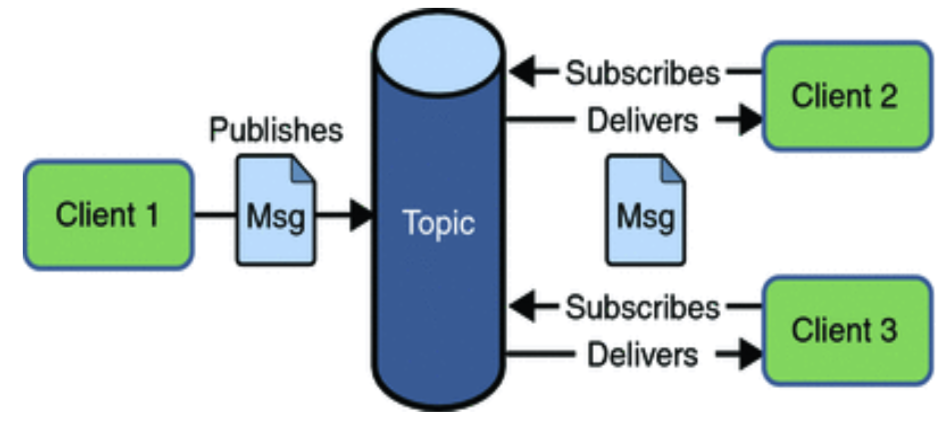
\includegraphics[width=0.7\textwidth]{ChatRoom}
\caption{The publish/subscribe model.}
\end{figure}

\begin{frm-def}[Topic]
In ROS, every message is sent using a topic. Some nodes send messages through the topic and other nodes receive messages through the topic. Topics are analogous to chat rooms.
\end{frm-def}

Topics are the medium in which nodes exchange messages in ROS. A node sends a message to a topic and any node that subscribes to that topic receives the message. In Figure 2.2, "Client 1" sends a message (publishes) to the topic and since both "Client 2" and "Client 3" listen (subscribe) to that topic, they will both receive the message. In ROS, these "clients" are nodes.

{\it Note: Topics can have any number of publishers and subscribers. Typically, having multiple publishers on a topic is a mistake.} \\

\begin{frm-def}[Publisher]
A publisher is a node that sends messages through a topic.
\end{frm-def}

Publishers are nodes that "publish" messages to a topic for other nodes to receive. These publisher nodes could be sensors that are transmitting data such as force or temperature. They might also be a controller sending out commands to control the motion of the robot. The publisher sends its messages with no regard for what nodes, if any, are looking for the message. Referring again to Figure 2.2, "Client 1" is the publisher.

{\it Note: If no nodes are subscribed to a published message, ROS automatically does not publish the unused data to preserve bandwidth.} \\

\begin{frm-def}[Subscriber]
A subscriber is a node that receives messages through a topic.
\end{frm-def}

When sensors or other publishers send their messages, there must be nodes to receive them. These nodes are called subscribers. They "subscribe" to a topic to receive relevant information in order to perform a task. For example, these subscribers might collect information from sensors to determine location or pass commands to control actuators. In Figure 2.2, "Client 2" and "Client 3" are subscribers receiving messages from the topic.\\

\section{Basics of programming with ROS}
\subsection{Creating a Publisher}
Starting a publisher consists of creating a node, setting a topic name, defining the type of message that will be sent, and setting a rate at which to send the message and a queue size for held messages. Nodes must have unique names; specifying the 'anonymous' option in node initialization allows the use of identical copies of a node, adding anonymous appendages to their names for uniqueness.
Sample code for creating a publisher node named "talker" is given below. The topic is "chatter" and it sends a string once per second.

\begin{verbatim}
import rospy
from std_msgs.msg import String

def talker():
    rospy.init_node('talker', anonymous=True)
    #create a node. 'talker' indicates that this node publishes.
    #The anonymous setting allows the master to check whether that name exists
    #already on the network and appends characters to make the name unique.

    pub.rospy.Publisher('chatter', String, queue_size=10)
    #chatter is the topic name, the message type is a string,
    #and there can be 10 messages in the queue

    rate = rospy.Rate(1)
    #sets the rate to 1 Hz. A message will be sent approximately once per second

    rospy.loginfo("Starting ROS node talker...")
    #this message sends when the publisher node starts up

    while not rospy.is_shutdown(): #as long as ROS is still running
        msg = "Greetings humans!" #define a message to send
        pub.publish(msg) #send the message
        rate.sleep() #wait until it is time to go again, defined by rate

if __name__ == '__main__':
    try:
        talker() #run the above function
    except rospy.ROSInterruptException: #if there is an error
        pass #this ignores the error. Often something else would be here

\end{verbatim}

Another option available when creating a publisher is the "latch." This allows a new subscriber to receive the last message sent. It can be useful for messages that are only sent once or very infrequently to allow new subscribers to receive the message without waiting for another update.

\subsection{Running the Node and Monitoring Messages}
% I think a section on how to get information from the command line might be useful. Things like the subscriber thing shown in lecture
% going to get the stuff from the video tomorrow (Sunday) and fill this in - Patrick
% re-arranged section headings around a bit and so added to this sub-section: let me know how this reads/ feel free to edit - Dipti
% I think command line things should come after we introduce the components, like it was before
The command 'rosrun' can be used to fire up this publisher node by specifying its name and the package it belongs to (more on packages later): for instance,
\begin{verbatim}
	rosrun aa274 talker.py
\end{verbatim}
As noted above, however, a publisher does not send messages until the topic is actually subscribed to. The rostopic command line tool offers a handy way to subscribe to a topic to monitor its messages. Below we list three most common rostopic commands:\\ \\
{\ttfamily
\begin{tabular}{l l}
rostopic list & lists all active topics \\
rostopic echo $<topic>$ & prints messages received on topic \\
rostopic hz $<topic>$ & measures topic publishing rate \\
\end{tabular}
}

The last command is particularly useful in debugging responsiveness of an application, for example in the face of a lossy connection in deep learning vision work.

\subsection{Creating a Subscriber}
Much like the publisher definition above, A subscriber node needs a subscriber function, specifying the topic name, message type, and a handle to a callback function. This callback function takes the incoming message as a parameter and performs some operation, such as printing the message data. The sample program below creates a subscriber node 'listener' that subscribes to the 'chatter' topic published by the 'talker' node.
\begin{verbatim}
import rospy
from std_msgs.msg import String

def callback(msg):
    rospy.loginfo("Received: %s", msg.data)
    #record the message as received

def listener():
    rospy.init_node('listener', anonymous=True)
    #create a node. 'listener' indicates that this node subscribes.
    #The anonymous setting allows the master to append characters to make the name unique.

    rospy.Subscriber("chatter", String, callback)
    #subscribe to the "chatter" topic, receiving Strings.
    #callback is filled by the above function

    rospy.loginfo("Listening on the chatter topic...")
    #indicate that the subscriber has started

    rospy.spin()
    #keep listening for messages

if __name__ == '__main__':
	listener()
\end{verbatim}

\subsection{Launch Files}
The launch file can be seen as the ROS notion of an application: instead of separately launching each subscriber and publisher node, ROS programmers can create Extensible Markup Language (XML) launch files to simultaneously start the master, execute multiple nodes, and set node parameters in a single executable. A simple example is given below. It starts with a comment to describe the file. Then, it creates a node with the name "talker" in the package "aa274" that outputs to the screen 5 times per second.
\begin{verbatim}
<launch>
    <!-- Start the talker node -->
    <node name="talker" pkg="aa274" type="talker.py" output="screen">
        <param name="rate" value="5"/>
    </node>
</launch>
\end{verbatim}

\subsection{Case Study using USB Camera}
An example of a more complex application of ROS is shown in class through the case study of edge detection in a camera image. A camera node connects to a USB camera, publishing raw images. An edge detection node runs on these raw images and publishes its processed images. Image view nodes subscribe to and display both images. A single launch file, shown below, launches all the nodes. An rqt\verb|_|graph, shown in Figure 2.3, helps visualize the connections between various publishers and subscribers. This case study demonstrates how a complex function can be accomplished simply by launching pre-existing nodes in ROS.

\begin{verbatim}
<launch>
    <arg name="video_device" default="/dev/video0" />

    <include file="$(find aa274)/launch/usbcam_driver.launch">
        <arg name="video_device" value="$(arg video_device)" />
    </include>

    <node name="image_view_1" pkg="image_view" type="image_view">
        <remap from="image" to="/camera/image_color" />
        <param name="autosize" value="true"/>
    </node>

    <node name="image_view_2" pkg="image_view" type="image_view">
        <remap from="image" to="/edge_detection/image" />
        <param name="autosize" value="true" />
    </node>

    <node name="edge_detection" pkg="opencv_apps" type="edge_detection">
        <remap from="image" to="/camera/image_color" />
        <param name="debug_view" value="false" />
    </node>
</launch>
\end{verbatim}

\begin{figure}[ht]
\centering
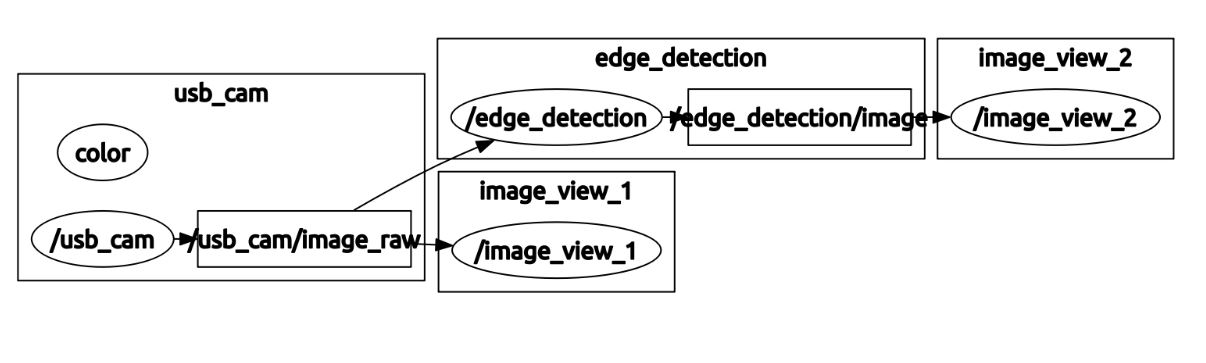
\includegraphics[width=1\textwidth]{USBCamera}
\caption{rqt graph of the edge detection case study.}
\end{figure}

\section{Developing with ROS}
\subsection{Catkin and ROS Packages}
Catkin is a build system for ROS and a Catkin workspace can be used to organize python scripts, launch files, etc in the form of nodes and packages. It's built on top of CMake, with additional features to tackle the complex dependencies that arise with ROS. ROS Packages are collections of nodes usually corresponding to a functionality, e.g. SLAM, and serve as the basic organizational structure for nodes.
Initializing a Catkin workspace allows one to manage the building of packages in its src directory:

\begin{verbatim}
mkdir -p ~/catkin_ws/src
cd ~/catkin_ws
catkin_make
\end{verbatim}

When a Catkin package is created, it is initialized with a CMakeLists file and a package.xml. Besides these, one typically needs sub-folders for config files, launch files and scripts as shown in Figure 2.3. Additional sub-folders may be required for more complex packages.
\begin{figure}[ht]
\centering
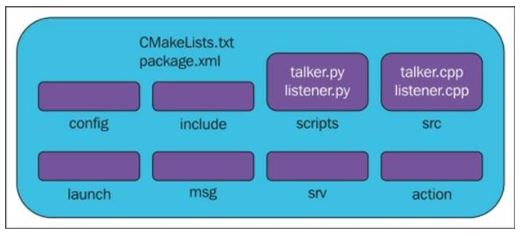
\includegraphics[width=0.8\textwidth]{ROSPackage}
\caption{The components of a typical ROS package in a Catkin workspace.}
\end{figure}

\subsection{Debugging}
Just as \verb|rostopic| enables us to monitor ROS topics in the command line, \verb|rospy.loginfo()| starts a background process that writes ROS messages to a ROS logger, viewable through a program such as \verb|rqt_console.|
Similarly, \verb|rosbag| provides a convenient way to record a number of topics for playback.

\subsection{Useful Features}
Custom Messages, ROS Services, Parameter Server and Dynamic Reconfigure are a few other useful features offered by ROS. ROS uses the Universal Robot Description Format (URDF) to specify the kinematic chain of robot models, allowing it to compute coordinate transforms between their different components. Gazebo is a (mostly) accurate physics simulator that is useful for testing code on a virtual robot.
\section{Getting Help}

There are many resources at your disposal for getting help with ROS. The following resources were mentioned in the slide-deck of this lecture:

\begin{itemize}
\item ROS wiki (http://wiki.ros.org/)
\item GitHub, Stack Overflow, and Google
\item The Construct / Robot Ignite Academy
\end{itemize}

\section{References}
About ROS. (2018). Retrieved from http://www.ros.org/about-ros/

Gazebo Robot Simulation. (2014). Retrieved from http://gazebosim.org/

\hangindent=2em
\hangafter=1
Goebel, P. (2013). \textit{ROS by Example}. Lulu. Retrieved from http://www.lulu.com/shop/r-patrick-goebel/ros-by-example-indigo-volume-1/ebook/product-22015937.html

Lentin, J. (2015). {\it Mastering ROS for robotics programming}. Birmingham, UK: Packt Publishing.

Open Source Robotics Foundation. (2018). Retrieved from https://www.osrfoundation.org/about/


\hangindent=2em
\hangafter=1
Pavone, M. (2018). {\it AA274: Principles of robotic autonomy, lecture 2 notes} [PowerPoint Slides]. Retrieved from https://canvas.stanford.edu/courses/75589/files/folder/Lectures?.

Willow Garage History. (2015). Retrieved from http://www.willowgarage.com/pages/about-us/history


\subsubsection{Contributors}
Winter 2019: [Your Names Here]
\\
Winter 2018: Marco Hinojosa, Ryan Loper, John McNelly, Dipti Motwani, Patrick Washington
\end{document}
